\begin{figure}[!tb]
\centering
\definecolor{exRandom}{HTML}{777777}\definecolor{exTeacher}{HTML}{000000}\definecolor{exRules}{HTML}{CC79A7}\definecolor{exMsmarco}{HTML}{999999}\definecolor{exArctic}{HTML}{0072B2}\definecolor{exLinear}{HTML}{000000}\definecolor{exMLP}{HTML}{D55E00}\definecolor{exFT}{HTML}{009E73}\definecolor{exFTMLP}{HTML}{E69F00}%
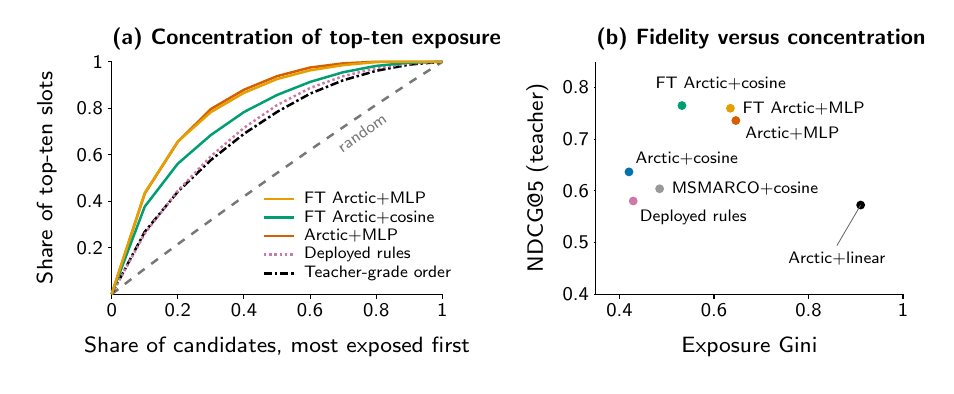
\begin{tikzpicture}[
  font=\fontsize{8}{9}\selectfont\sffamily,
  tick/.style={font=\fontsize{7}{8}\selectfont\sffamily, inner sep=1.5pt},
  plabel/.style={font=\fontsize{6}{7}\selectfont\sffamily, inner sep=1.2pt},
  curve/.style={line width=0.9pt, line join=round},
  title/.style={anchor=south west, inner sep=0pt,
    font=\fontsize{8}{9}\selectfont\sffamily\bfseries},
]
\begin{scope}[xshift=0.95cm, yshift=0.75cm, x=4.2cm, y=2.952cm]
  \draw[line width=0.4pt] (0,0) -- (1,0);
  \draw[line width=0.4pt] (0,0) -- (0,1);
  \foreach \x in {0,0.2,0.4,0.6,0.8,1}
    \draw (\x,0) -- (\x,-0.02) node[tick, below] {\x};
  \foreach \y in {0.2,0.4,0.6,0.8,1}
    \draw (0,\y) -- (-0.012,\y) node[tick, left] {\y};
  \draw[curve, exRandom, dashed] plot coordinates {(0,0.0000) (0.1,0.1094) (0.2,0.2150) (0.3,0.3185) (0.4,0.4205) (0.5,0.5212) (0.6,0.6206) (0.7,0.7185) (0.8,0.8151) (0.9,0.9092) (1,1.0000)};
  \draw[curve, exTeacher, densely dashdotted] plot coordinates {(0,-0.0000) (0.1,0.2683) (0.2,0.4408) (0.3,0.5771) (0.4,0.6899) (0.5,0.7841) (0.6,0.8627) (0.7,0.9203) (0.8,0.9610) (0.9,0.9878) (1,1.0000)};
  \draw[curve, exRules, densely dotted] plot coordinates {(0,0.0000) (0.1,0.2608) (0.2,0.4448) (0.3,0.5936) (0.4,0.7154) (0.5,0.8132) (0.6,0.8871) (0.7,0.9379) (0.8,0.9722) (0.9,0.9929) (1,1.0000)};
  \draw[curve, exMLP, solid] plot coordinates {(0,0.0000) (0.1,0.4329) (0.2,0.6556) (0.3,0.7966) (0.4,0.8794) (0.5,0.9379) (0.6,0.9751) (0.7,0.9930) (0.8,1.0000) (0.9,1.0000) (1,1.0000)};
  \draw[curve, exFT, solid] plot coordinates {(0,0.0000) (0.1,0.3767) (0.2,0.5615) (0.3,0.6848) (0.4,0.7835) (0.5,0.8570) (0.6,0.9132) (0.7,0.9549) (0.8,0.9822) (0.9,0.9959) (1,1.0000)};
  \draw[curve, exFTMLP, solid] plot coordinates {(0,0.0000) (0.1,0.4351) (0.2,0.6568) (0.3,0.7834) (0.4,0.8662) (0.5,0.9256) (0.6,0.9631) (0.7,0.9855) (0.8,0.9988) (0.9,1.0000) (1,1.0000)};
  \draw[curve, exFTMLP, solid] (0.46,0.41) -- ++(0.09,0);
  \node[plabel, anchor=west] at (0.57,0.41) {\model{FT Arctic+MLP}};
  \draw[curve, exFT, solid] (0.46,0.33) -- ++(0.09,0);
  \node[plabel, anchor=west] at (0.57,0.33) {\model{FT Arctic+cosine}};
  \draw[curve, exMLP, solid] (0.46,0.25) -- ++(0.09,0);
  \node[plabel, anchor=west] at (0.57,0.25) {\model{Arctic+MLP}};
  \draw[curve, exRules, densely dotted] (0.46,0.17) -- ++(0.09,0);
  \node[plabel, anchor=west] at (0.57,0.17) {Deployed rules};
  \draw[curve, exTeacher, densely dashdotted] (0.46,0.09) -- ++(0.09,0);
  \node[plabel, anchor=west] at (0.57,0.09) {Teacher-grade order};
  \node[plabel, rotate=35, anchor=north, text=exRandom] at (0.74,0.73) {random};
  \node[anchor=north] at (0.5,-0.142) {Share of candidates, most exposed first};
  \node[rotate=90, anchor=south] at (-0.137,0.5) {Share of top-ten slots};
  \node[title] at (0,1.049) {(a) Concentration of top-ten exposure};
\end{scope}
\begin{scope}[xshift=5.0cm, yshift=-1.874cm, x=6.0cm, y=6.56cm]
  \draw[line width=0.4pt] (0.35,0.40) -- (1,0.40);
  \draw[line width=0.4pt] (0.35,0.40) -- (0.35,0.85);
  \foreach \x in {0.4,0.6,0.8,1}
    \draw (\x,0.40) -- (\x,0.391) node[tick, below] {\x};
  \foreach \y in {0.4,0.5,0.6,0.7,0.8}
    \draw (0.35,\y) -- (0.345,\y) node[tick, left] {\y};
  \fill[exMsmarco] (0.4849,0.6041) circle (1.6pt);
  \node[plabel, anchor=west, xshift=3pt, yshift=0pt] at (0.4849,0.6041) {\model{MSMARCO+cosine}};
  \fill[exArctic] (0.4200,0.6368) circle (1.6pt);
  \node[plabel, anchor=south west, xshift=1pt, yshift=1pt] at (0.4200,0.6368) {\model{Arctic+cosine}};
  \fill[exRules] (0.4290,0.5804) circle (1.6pt);
  \node[plabel, anchor=north west, xshift=1pt, yshift=-2pt] at (0.4290,0.5804) {Deployed rules};
  \fill[exLinear] (0.9104,0.5726) circle (1.6pt);
  \draw[line width=0.3pt, black!60] (0.9104,0.5726) -- (0.86,0.494);
  \node[plabel, anchor=north] at (0.86,0.49) {\model{Arctic+linear}};
  \fill[exMLP] (0.6462,0.7362) circle (1.6pt);
  \node[plabel, anchor=north west, xshift=2pt, yshift=-1pt] at (0.6462,0.7362) {\model{Arctic+MLP}};
  \fill[exFT] (0.5321,0.7652) circle (1.6pt);
  \node[plabel, anchor=south, xshift=14pt, yshift=4pt] at (0.5321,0.7652) {\model{FT Arctic+cosine}};
  \fill[exFTMLP] (0.6347,0.7599) circle (1.6pt);
  \node[plabel, anchor=west, xshift=3pt, yshift=0pt] at (0.6347,0.7599) {\model{FT Arctic+MLP}};
  \node[anchor=north] at (0.675,0.336) {Exposure Gini};
  \node[rotate=90, anchor=south] at (0.27,0.625) {NDCG@5 (teacher)};
  \node[title] at (0.35,0.872) {(b) Fidelity versus concentration};
\end{scope}
\end{tikzpicture}
\Description{Two panels for the 356 test users. Left: share of top-ten slots held by the most-exposed share of candidates. Random expected exposure follows the diagonal; ordering by the teacher's grades and the deployed rules concentrate least, the fine-tuned cosine retriever more, and the two MLP students most. Right: scatter of teacher NDCG@5 against exposure Gini. The fine-tuned cosine retriever has the highest NDCG@5 with a Gini near 0.53; the MLP students reach similar NDCG@5 with Gini near 0.64; the linear scorer on concatenated embeddings has low NDCG@5 and a Gini of 0.91; the deployed rules and pretrained cosine models have NDCG@5 between 0.58 and 0.64 and Gini between 0.42 and 0.49.}

\caption{Exposure on the test lists (356 users). (a) Share of top-ten slots held by the
most-exposed candidates (deciles; ties averaged, random expected); pretrained
\model{Arctic+cosine} lies on the rules' curve. (b) Teacher NDCG@5
(Table~\ref{tab:fidelity-ecir}) against exposure Gini for each scorer.}
\label{fig:exposure}
\end{figure}
